% !TEX root = ../my-thesis.tex
%

\chapter{Banc de test}
\label{sec:Benchmark}

%\cleanchapterquote{Un petit chapitre pour le doctorant, un grand chapitre pour l'humanité}{Doctorant anonyme}{(Citation temporaire)}

\section{Motivations}
\label{sec:Benchmark:Motivations}


Comme nous l'avons conclu dans le chapitre précédent, se baser sur la littérature dans le but de choisir un filtre de rehaussement pour une application spécifique n'est pas une tâche simple. La littérature permet de se faire une vision globale sur les filtres de rehaussement de vaisseaux sanguins et présente de nombreux exemples d'applications. Cependant, leur incorporation dans une chaîne de traitements dilue l'évaluation de leur impact réel sur la segmentation. Elle rend aussi plus difficile le choix d'un filtre et ses paramètres optimaux pour une modalité et un organe spécifiques. De plus, les métriques de références varient aussi entre deux publications ajoutant à la difficulté d'établir une comparaison. Il est donc nécessaire de proposer une base de
 comparaison unifiée (Fig. \ref{fig:problematics}).

\begin{figure}[!ht]
  \centering
  \adjincludegraphics[width=0.32\textwidth,trim={{0.12\width} {0.1\height} {0\width} {0.1\height}},clip]{Images/filters_variation_gt.png}
\\
  \adjincludegraphics[width=0.32\textwidth,trim={{0.12\width} {0.1\height} {0\width} {0.1\height}},clip]{Images/antiga_02_08_15.png}
  \adjincludegraphics[width=0.32\textwidth,trim={{0.12\width} {0.1\height} {0\width} {0.1\height}},clip]{Images/antiga_05_05_15.png}
  \adjincludegraphics[width=0.32\textwidth,trim={{0.12\width} {0.1\height} {0\width} {0.1\height}},clip]{Images/antiga_07_03_15.png}
  \\
  \adjincludegraphics[width=0.32\textwidth,trim={{0.12\width} {0.1\height} {0\width} {0.1\height}},clip]{Images/jerman_1.png}
  \adjincludegraphics[width=0.32\textwidth,trim={{0.12\width} {0.1\height} {0\width} {0.1\height}},clip]{Images/jerman_04.png}
  \adjincludegraphics[width=0.32\textwidth,trim={{0.12\width} {0.1\height} {0\width} {0.1\height}},clip]{Images/jerman_01.png}
  \\
  %missing RORPO_50_15_4.png....
  \adjincludegraphics[width=0.32\textwidth,trim={{0.12\width} {0.1\height} {0\width} {0.1\height}},clip]{Images/img_required.jpg}
  \adjincludegraphics[width=0.32\textwidth,trim={{0.12\width} {0.1\height} {0\width} {0.1\height}},clip]{Images/RORPO_51_25_3.png}
  \adjincludegraphics[width=0.32\textwidth,trim={{0.12\width} {0.1\height} {0\width} {0.1\height}},clip]{Images/RORPO_100_15_3.png}
  \caption{Illustration de l'application de différents filtres et jeux de paramètres. La première ligne montre la vérité terrain. Les lignes suivantes montrent ligne par ligne les filtres de Frangi, Jerman et RORPO. Il est difficile de choisir laquelle de ces paramétrisations est la plus apte pour une segmentation sans évaluation quantitative.}
  \label{fig:problematics}
\end{figure}

Dans ce chapitre, nous abordons la conception d'un banc de test permettant l'étude quantitative des filtres de rehaussement. Notre banc de test permet d'appliquer plusieurs instances de paramètres d'un filtre sur une base de données. Le résultat du filtrage est ensuite seuillé et les métriques d'évaluations sont calculées dans des zones d'intérêt définies par l'utilisateur. Une fois les métriques collectées, celles-ci peuvent être exploitées indépendamment par des outils de traitement de données. Son fonctionnement est illustré dans la Fig. \ref{fig:schéma banc de test}

La création de notre banc de test passe par la construction d'une interface de filtres unifiée, la construction des jeux de données, la création de zones d'évaluation et le choix des métriques d'évaluation. Cette construction s'est réalisée de manière itérative au fur et à mesure des observations faites durant les expériences dont les résultats sont présentés dans le chapitre 4.

\tikzstyle{capNode} = [rectangle, rounded corners, minimum width=3cm, minimum height=1cm,text centered, draw=black]
\tikzstyle{capNodeRed} = [rectangle, rounded corners, minimum width=3cm, minimum height=1cm,text centered, draw=red]
\tikzstyle{cNode} = [circle, minimum width=1cm, minimum height=1cm, text centered, draw=black, fill=white!30]
\tikzstyle{arrow} = [thick,->,>=stealth]

\begin{figure}[!ht]
  \centering
  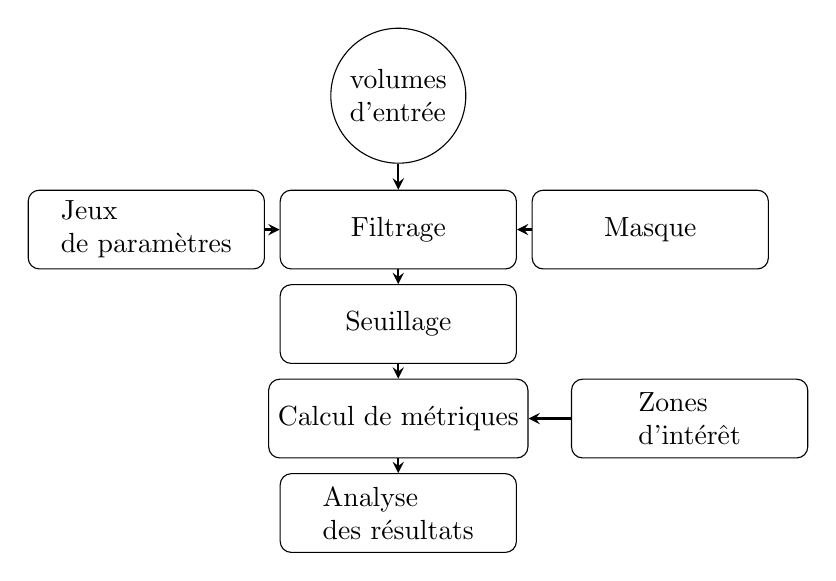
\begin{tikzpicture}[node distance=1.2cm]
    \node (input)[cNode,align=left] {volumes \\ d'entrée};
    \node (filtrage)[capNode, below of=input,align=left,yshift=-0.5cm] {Filtrage};
    \node (parametres)[capNode, left of=filtrage,align=left,xshift=-2cm] {Jeux \\ de paramètres};
    \node (Masques)[capNode, right of=filtrage,align=left,xshift=2cm] {Masque};
    \node (seuillage)[capNode, below of=filtrage, align=left] {Seuillage};
    \node (metriques)[capNode, below of=seuillage, align=left] {Calcul de métriques};
    \node (ZI)[capNode, right of=metriques, align=left,xshift=2.5cm] {Zones \\ d'intérêt};
    \node (traitement)[capNode, below of=metriques, align=left] {Analyse \\ des résultats};
  
    \draw [arrow] (input) -- (filtrage);
    \draw [arrow] (filtrage) -- (seuillage);
    \draw [arrow] (parametres) -- (filtrage);
    \draw [arrow] (Masques) -- (filtrage);
    \draw [arrow] (ZI) -- (metriques);
    \draw [arrow] (seuillage) -- (metriques);
    \draw [arrow] (metriques) -- (traitement);

  \end{tikzpicture}
  \caption{Schéma global du banc de test. Celui-ci présente une architecture simple afin de faciliter la prise en main par d'autres utilisateurs.}
  \label{fig:schéma banc de test}
\end{figure}

\section{Travaux existants}

 Quelques travaux proposent une comparaison entre filtres de rehaussement. Par exemple Obara, Sazak et Alharbi et al. \cite{Alharbi2018_TP_2D_3D} \cite{Sazak2019_bowler_hat_2D}  ont proposé une méthode de rehaussement de vaisseaux à base de morphologie mathématique en 2D et 3D. Ce filtre est comparé à d'autres filtres 2D et 3D à base de hessiennes ou de tenseurs de phase. Ces articles donnent toutefois une part importante à l'évaluation qualitative plutôt que quantitative. De plus, ils ne proposent pas de discussion sur l'impact de la paramétrisation des filtres. En 3D, une analyse quantitative des filtres de rehaussement sur un grand nombre de volumes a été réalisée par Manh Luu en 2015 \cite{Luu2015_liver_vesselness_comparison} et Phellan \cite{Phellan2017_Brain_vesselness_comparison} en 2017. Manh Luu avait rendu ses travaux publics, cependant le site internet n'est aujourd'hui plus accessible.

Manh Luu et al. \cite{Luu2015_liver_vesselness_comparison} ont proposé un banc de test sur 51 images tomodensitométriques du foie sans prétraitement des données. Ils ajoutent cependant une segmentation à base de croissance de région dans leur chaîne de traitement et une fermeture morphologique pour supprimer les composantes connexes inférieures à 10 voxels. Dans leurs travaux, l'évaluation de la qualité de la segmentation est basée sur des échantillons de marqueurs positionnés manuellement à l'intérieur et autour des vaisseaux (Fig. \ref{fig:ManhLuu_markers}). Entre 300 et 700 points par volumes sont annotés à l'intérieur des vaisseaux et 4 marqueurs du voisinage des vaisseaux sont ajoutés par points internes. Les filtres testés sont Frangi, Sato, Erdt et les schémas de diffusion HDCS (\textit{Hybrid Diffusion with Continuous Switch}), VED (\textit{Vessel Enhancement Diffusion}) et RPM (\textit{Regularized Perona-Malik}). Les paramètres des filtres sont optimisés sur une sous-section de la base de données. L'optimisation des paramètres est un fait suffisamment rare dans la littérature pour être souligné. Les métriques utilisées pour l'évaluation des filtres sont le rapport signal sur bruit (SNR), le rappel, la précision (accuracy) et la spécificité.

\begin{figure}[!ht]
  \centering
  \includegraphics[height=6cm]{Images/ManhLuu_markers.png}
  \caption{Marqueurs utilisés par Manh Luu et al. En rouge, marqueurs de vaisseaux, en vert, marqueurs extérieurs aux vaisseaux. Image issue de \cite{Luu2015_liver_vesselness_comparison}. }
  \label{fig:ManhLuu_markers}
\end{figure}

Phellan et al. proposent quant à eux un banc de test sur 5 images IRM du cerveau et 40 volumes générés avec VascuSynth et l'ajout d'artefacts de tomodensitométrie. Leur chaîne de traitement inclut un prétraitement des données et une segmentation à base de seuillages et d'un filtrage de composantes connexes. Leur méthode d'analyse repose sur des vérités terrains binaires du réseau vasculaire entier et sur l'évaluation du diamètre des vaisseaux. De plus, Phellan et al. considèrent que la détection est plus importante que la précision des contours à l'étape du rehaussement. Ils définissent donc une zone d'acceptation dans laquelle les voxels ne participent pas à la métrique (Fig. \ref{fig:Phellan_acceptance_zone}). Les filtres évalués par Phellan sont Frangi, Sato, Erdt, OOF, RORPO, WTH et les schémas de diffusion HDCS, VED et RPM. Seuls les paramètres d'échelle sont optimisés dans ces travaux, les paramètres intrinsèques par défaut étant fixé par les auteurs. Les performances des filtres sont évaluées grâce au Dice, au MCC, à l'analyse de courbes ROC et à travers une analyse des composantes connexes.

\begin{figure}[!ht]
  \centering
  \includegraphics[height=4cm]{Images/Phellan_comparison.jpg}
  \caption{Zone d'acceptation de Phellan définie comme la zone entre l'érosion (gris) et la dilatation (blanc) de la vérité terrain. La bordure réelle des vaisseaux se situe au sein de la zone blanche, mais les métriques ne sont calculées que dans la zone grise. Cette méthode exclut une partie des petits vaisseaux.}
  \label{fig:Phellan_acceptance_zone}
\end{figure}

Ces deux bancs de test proposent des méthodes d'évaluations différentes. Pour notre application, des points intéressants sont présents dans les deux benchmarks, qui chacun recouvre une partie de nos besoins sans toutefois y répondre complètement. En effet, l'évaluation de Manh Luu sur le foie n'est pas faite sur une segmentation voxélique. Cette évaluation éparse, en quelques points dans le voisinage des vaisseaux peut mésestimer des artefacts comme un rehaussement bruité à la surface des vaisseaux. Le travail de Phellan est réalisé sur un autre organe sans optimisation des paramètres. Des filtres récents ne sont pas évalués, car ils sont postérieurs aux publications. 

Nous souhaitions fortement pouvoir évaluer les filtres sur des zones spécifiques définies par l'utilisateur telles que les bifurcations des vaisseaux. Ces zones sont en effet connues pour être plus faiblement rehaussées sans que la littérature n'apporte de résultats quantifiables. Une analyse du rehaussement par taille de vaisseaux n'est pas non plus disponible pour le foie. C'est pourquoi nous avons voulu créer notre propre banc de test, orienté vers l'imagerie du foie. Nous avons voulu éviter d'effectuer les mêmes erreurs que les travaux précédents en proposant une base suffisamment globale pour s'accommoder de différentes modalités et suffisamment modulaire pour être utilisées dans diverses expériences afin que la prise en main par d'autres utilisateurs soit possible.

\section{Homogénéisation des filtres}
\label{sec:Filtres}

Former une base homogène de filtres n'est pas une tâche simple. Celle-ci nécessite la recherche de code existant ou d'implémenter les filtres en se basant sur la méthodologie de l'article original.

Réaliser l'implémentation d'un filtre à partir des indications de l'auteur est parfois complexe, car il doit souvent se soumettre à un exercice de concision lors de la publication de ses travaux. L'auteur va donc à l'essentiel et certains détails d'implémentation peuvent être omis. La difficulté peut aussi survenir d'un problème de compréhension de la part du lecteur, surtout lorsque les articles sont écrits dans une langue étrangère à la sienne. Il faut donc être particulièrement attentif à la compréhension et à la vérification des hypothèses afin d'implémenter correctement les filtres. 

La collecte d'implémentations existantes n'est pas non plus évidente. En effet, il est possible que plusieurs versions d'un algorithme existent. Il est alors nécessaire de vérifier le code en détail. Certaines implémentations peuvent présenter des interfaces différentes de l'article original et nécessiter un travail de traduction d'une interface à l'autre. Il arrive aussi que des codes soient disponibles, mais avec une dette technologique importante suite à l'évolution des logiciels ou des librairies nécessaires à leur fonctionnement. Il est possible aussi que des implémentations ajoutent des améliorations non documentées dans les articles originaux, ce qui peut être problématique dans les travaux de comparaison. Enfin, la multiplicité des langages, des librairies et des logiciels sur lesquels sont déployés les filtres ajoute au temps dédié à cette tâche. Ce travail est souvent réalisé de manière isolée par un chercheur, un doctorant, ou un stagiaire pour leurs expériences personnelles et ne profite pas à la communauté travaillant sur le sujet. Il doit alors reprendre de lui-même la totalité de ce travail à chaque introduction d'une nouvelle méthode.

Dans nos travaux, nous avons sélectionné, adapté et implémenté sept filtres qui répondent tous à une problématique spécifique du rehaussement (Tab. \ref{Tab:available_vesselness}). La diversité de leur origine est résumée dans la table \ref{Tab:origins_vesselness}. Il a été choisi d'implémenter ces filtres et d'effectuer les modifications nécessaires pour les filtres existants en C++ avec la librairie ITK. Le C++ est particulièrement connu pour sa rapidité, un élément crucial pour des applications 3D qui doivent traiter un nombre important de voxels. La librairie open source ITK (Insight ToolKit), développée par Kitware Inc. depuis 2001, est la plus importante librairie de traitement d'images médicales. Elle fournit un ensemble de briques algorithmiques déjà implémentées et présente l'avantage de lire nativement une grande diversité de formats d'images médicales, ce qui est un atout pour la diffusion de notre banc de test.

Cette librairie s'appuie sur une communauté active et connait des mises à jour régulières. C'est à la fois un avantage, pour la correction de bugs et l'introduction de nouveaux algorithmes mais aussi un inconvénient, car la dette technologique s'accumule plus rapidement à cause de cycles plus courts entre deux versions.


\begin{table}
    \begin{center}
      \resizebox{\textwidth}{!}{
  \begin{tabular}{l|l|l}
  Méthode   &  Idée centrale                                                                       & Date \\ \hline  \hline 
  Sato      & Reconnexion des vaisseaux, contrôle du bruit                                         & 1997 \\ \hline
  Frangi    & Contrôle sur l'atténuation des structures en plateau et en blob                     & 1998 \\ \hline
  Meijering & Détection de fines structures allongées                                             & 2004 \\ \hline
  OOF       & Limitation du débordement des réponses lié à l'espace d'échelles gaussien             & 2010 \\ \hline
  Jerman    & Contrôle de l'homogénéité des réponses des vaisseaux                                 & 2016 \\ \hline
  Zhang     & Pré-traitement pour limiter le rehaussement des bordures du foie (TDM foie)          & 2018 \\ \hline
  RORPO     & Détection par chemins et différentiation des vaisseaux par vote sur les orientations & 2018  
  \end{tabular}
  }
  \end{center}
  \caption{Méthodes disponibles et idées principales guidant leur conception.}
  \label{Tab:available_vesselness}

  \end{table}

  \begin{table}
    \begin{center}
      \resizebox{\textwidth}{!}{
        \begin{tabular}{l|l|l|l}
            Méthode   &  Provenance                                     & État \\ \hline  \hline 
            Sato      & Librairie ITK (C++)                             & prêt à l'emploi \\ \hline
            Frangi    & Librairie ITK (C++)                             & prêt à l'emploi \\ \hline
            Meijering & Github (Matlab), scipy                          & pondération proposée ne respectant pas l'article original.  \\ \hline
            OOF       & Site de l'auteur (Matlab), insight journal (C++)& obsolète \\ \hline
            Jerman    & Github de l'auteur (Matlab)                     & prêt à l'emploi \\ \hline
            Zhang     & Non disponible                                  & non implémenté \\ \hline
            RORPO     & Github de l'auteur (C++)                        & prêt à l'emploi  
        \end{tabular}
      }
    \end{center}
    \caption{Origine des méthodes. La diversité des provenances et l'ancienneté du code complique la mise en oeuvre d'une comparaison des filtres.}
    \label{Tab:origins_vesselness}
  \end{table}

La conception de notre banc de test a été guidée par plusieurs axes majeurs.
  
Le premier axe de conception a été d'évaluer le rehaussement pour la segmentation voxélique. L'analyse à partir d'un ensemble de marqueurs comme réalisé par Manh Luu nous a paru trop éparse pour rendre compte de la totalité du profil du rehaussement. Nous avons aussi voulu éviter au maximum des traitements supplémentaire avant et après le rehaussement afin d'évaluer au plus près les filtres. La segmentation voxélique s'imposait donc comme le meilleur choix. La nature voxélique des vérités terrains des jeux de données disponibles et une plus grande quantité d'applications annexes (maillages, simulation de flux) pouvant servir au projet R-Vessel-X  nous a conforté dans ce choix.

\subsection{Redéfinition du domaine de sortie des filtres}

Le rehaussement de vaisseaux est parfois présenté comme une carte chaleur ou de probabilité pour laquelle une quantité d'appartenance à un vaisseau est associée à chaque voxel. Pour le filtre de Frangi, cette quantité est définie entre 0 et 1. Cette propriété est souhaitable dans de nombreuses applications, car elle est plus simple à intégrer dans des chaînes de traitement que des filtres définis sur des domaines plus larges. Elle est aussi plus simple à interpréter.

Cependant, la réponse de tous les filtres ne partage pas nécessairement cette propriété. Par construction, seuls Jerman, Zhang et Meijering fournissent une réponse définie sur cet intervalle. La réponse de Sato est définie sur $[0,+\infty]$, tout comme celle d'OOF. RORPO est un cas particulier, car l'intensité de sortie du filtre dépend de l'intensité maximum de l'image source. En effet, RORPO se base sur des ouvertures morphologiques dont la définition est bornée par le domaine de l'image. 

Dans une optique de généralisation et de diffusion des filtres, nous partons du principe que les images des bases de données ne sont pas normalisées. On ne peut donc pas espérer une stabilité des sorties de chaque filtre à partir de leur entrée. Il faut par conséquent contraindre les sorties des filtres entre zéro et un. Nous avons choisi pour Sato et OOF de normaliser la réponse de sortie en fonction de la plus grande valeur de sortie du filtre :

\begin{equation}
  \frac{I_{rehaussement}(x)} {\max(I{rehaussement}(x))}
\end{equation}

Pour RORPO dont la sortie est liée à l'intensité de l'image d'entrée, la normalisation prend la forme $ \frac{I_{rehaussement}(x)} {\max(I(x))} $.
La nature de RORPO en fait un filtre difficile à intégrer à notre banc de test. En effet, l'utilisation de la morphologie implique une utilisation ``tout ou rien'', à mi-chemin entre segmentation binaire et rehaussement. On conserve en effet seulement les intensités des voxels candidats à la participation de structures tubulaires sans leur associer de degré d'appartenance. Cette segmentation en niveaux de gris force l'utilisation d'une normalisation non naturelle pour passer à une carte de probabilité nécessaire pour l'évaluation de ce benchmark. Cette procédure a un impact non négligeable sur le résultat des expériences présentées dans le chapitre suivant.

Une attention particulière doit être portée aux types d'images pris en charge par l'implémentation des filtres. En effet, la dynamique des images médicales n'est pas commune. Une image 2D classique est souvent représentée sur 8 bits exprimant 256 niveaux de gris $[0,255]$ (mis à la puissance 3 les images couleurs). Les images médicales possèdent la plupart du temps un seul canal avec parfois une dynamique de niveaux de gris plus importante de 16 ou 32 bits et peuvent présenter des valeurs négatives comme pour la tomodensitométrie présentée au Chap. 2. Il faut donc s'assurer que les filtres prennent bien en compte les mêmes types d’images. Un même filtre peut en effet produire des résultats différents selon la précision des images (8 bits vs. 32 bits). Par exemple, l'implémentation de RORPO ne supporte que des valeurs de pixels positifs et nécessite de faire une translation des niveaux de gris négatifs sous peine d'obtenir des comportements non définis.

\subsection{Utilisation de masques}

Il peut souvent être utile de ne traiter qu'une partie de l'image, par exemple lorsque l'utilisateur ne veut rehausser les vaisseaux que d'un organe en particulier. La manière la plus simple est de définir un masque binaire de taille équivalente à l'image. On renseigne pour chaque voxel s'il appartient à la zone à traiter (1 ou 255) ou s'il n'y appartient pas (0). Là encore, il faut être attentif à l'implémentation du masque, car le positionnement (Fig. \ref{fig:masks_posible_location}) du masque peut impacter les performances des filtres. Une première implémentation consiste à appliquer le masque sur le rehaussement en aval de celui-ci. Le filtre est appliqué à toute l'image avant de ne conserver que la partie concernant l'organe observé. Cette implémentation a le désavantage de calculer le rehaussement dans des zones non utilisées par la suite, telles que les zones avec un faible bruit autour du corps du patient. Une seconde implémentation consiste à masquer l'image dans un premier temps, puis à calculer le rehaussement dans cette image masquée. On gagne ainsi du temps de calcul dans les zones à valeurs nulles qui ne font pas partie de l'évaluation. Ce gain de temps n'est pas négligeable, puisqu'un banc de test applique de multiples fois les filtres sur un grand nombre de volumes 3D. Cependant, masquer en aval du rehaussement crée artificiellement de faux bords en induisant un différentiel d'intensités marqué (voir Fig. \ref{fig:mask_intensity_profile}).
 
\begin{figure}[!ht]
  \centering
  \includegraphics[height=4cm]{Images/output_maskedFirst.png}
  \includegraphics[height=4cm]{Images/output_unmasked.png}
  \includegraphics[height=4cm]{Images/output_masking_diff.png}
  \caption{Rehaussement avec masque en amont (gauche) et masque en aval (droite). La différence (fond gris) des deux masques est visible au centre. Le masque en amont crée un contour artificiellement nette que le filtre rehausse.}
  \label{fig:mask_intensity_profile}
\end{figure}

De plus, on se heurte à un problème pour les filtres à information globale. On peut en effet classer les filtres de rehaussement en deux catégories. Les filtres à seule information locale et les filtres à information locale et globale. Les filtres à information locale ne considèrent le rehaussement que par rapport à des mesures effectuées dans un voisinage local. Ce voisinage est défini par la taille de la gaussienne pour les méthodes à espace d'échelles gaussien et par la taille de l'élément structurant pour les méthodes à base de morphologie. Les filtres à information locale sont Frangi, Sato, RORPO et OOF.

Les filtres à information globale sont Meijering, Jerman et Zhang. Meijering et Jerman/Zhang nécessitent la plus petite valeur propre (équivalent à la plus grande valeur propre négative en valeur absolue) de la zone sur laquelle est appliqué le rehaussement. Le pré-filtrage de Zhang nécessite lui aussi une information globale puisque cette étape repose sur la classification de l'ensemble des pixels de la zone de rehaussement. Dans le cas de ces filtres, une intégration naïve des masques a un impact critique sur le résultat du rehaussement. En effet, une image de l'abdomen contient aussi les os de la cage thoracique qui possèdent une intensité largement supérieure aux vaisseaux du foie en TDM. Dans le cas d'un filtre à information globale comme le filtre de Jerman, la mesure de rehaussement sera pondérée par les valeurs propres minimales de l'image, donc celle des os (structures intenses), et non celles des vaisseaux. 

Une stratégie de masque a donc été choisie spécifiquement pour chaque filtre. Ainsi pour Frangi, Sato, OOF, RORPO, le masque est appliqué en aval du rehaussement, cela afin de limiter l'introduction de faux gradients liés au masque. Pour les autres filtres, une stratégie plus complexe a été utilisée.

Comme nous avons implémenté nous-même les filtres de Jerman, Meijering et Zhang, nous pouvons avoir un contrôle plus fin sur l'étape d'application du masque. Afin de combiner les deux propriétés de limitation du temps de calcul et de non-introduction de bordures nettes artificielles, l'opération de masque est introduite entre le calcul de la matrice hessienne et le calcul de ses valeurs propres. Ne sont calculées les valeurs propres que des pixels appartenant au masque tout en calculant la matrice hessienne sur la globalité du volume. On obtient ainsi un compromis tirant parti des avantages entre masque en amont et masque en aval (voir Fig. \ref{fig:smart_mask_effect}).

\begin{figure}[!ht]
  \centering
  \includegraphics[height=4cm]{Images/globInfo_noM_loc.png}
  \includegraphics[height=4cm]{Images/globInfo_M_loc.png}
  \includegraphics[height=4cm]{Images/globInfo_noM_glob.png}
  \caption{Première ligne : à gauche, filtre de Jerman avec masque en aval. À droite, filtre de Jerman avec masque en amont. Seconde ligne : rehaussement avant l'application du masque en aval. La limite haute du rehaussement est définie par les structures intenses hors du foie plutôt que par les vaisseaux hépatiques. Dans les deux cas, les mêmes paramètres ont été appliqués.}
  \label{fig:smart_mask_effect}
\end{figure}

\begin{figure}[!ht]

    \centering
    %\resizebox{\linewidth}{
      
  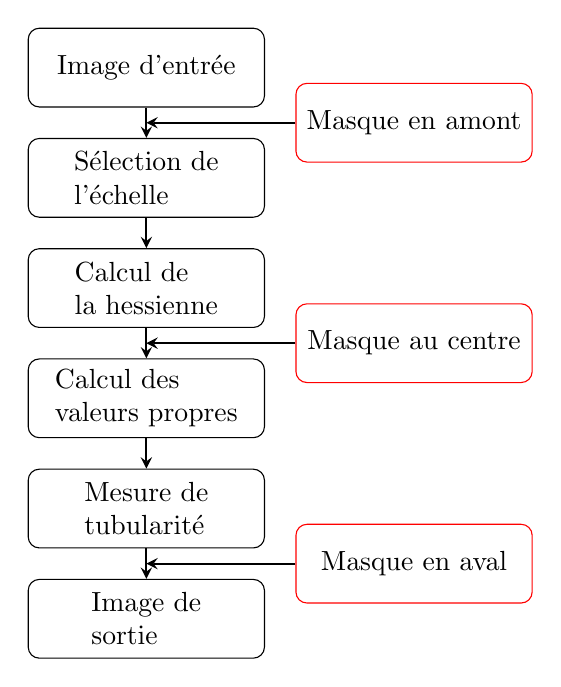
\begin{tikzpicture}[node distance=1.4cm]
    \node (input)[capNode] {Image d'entrée};
    \node (scale_selection)[capNode, below of=input,align=left] {Sélection de \\ l'échelle};
    \node (hessian)[capNode, below of=scale_selection,align=left] {Calcul de \\ la hessienne};
    \node (EV)[capNode, below of=hessian,align=left] {Calcul des \\ valeurs propres};
    \node (vesselness)[capNode, below of=EV,align=left] {Mesure de \\ tubularité};
    \node (output)[capNode, below of=vesselness,align=left] {Image de \\ sortie};

    \draw [arrow] (input) -- (scale_selection) coordinate[midway] (a_input){};
    \draw [arrow] (scale_selection) -- (hessian) coordinate[midway] (a_sc){};
    \draw [arrow] (hessian) -- (EV) coordinate[midway] (a_hessian){};
    \draw [arrow] (EV) -- (vesselness) coordinate[midway] (a_EV){}; 
    \draw [arrow] (vesselness) -- (output) coordinate[midway] (a_Vesselness){};

    \node (p1)[capNodeRed,right of=a_input,xshift=2cm]{Masque en amont};
    \node (p2)[capNodeRed,right of=a_hessian,xshift=2cm]{Masque au centre};
    \node (p3)[capNodeRed,right of=a_Vesselness,xshift=2cm]{Masque en aval};

    \draw [arrow] (p1) -- (a_input);
    \draw [arrow] (p2) -- (a_hessian);
    \draw [arrow] (p3) -- (a_Vesselness);

    %\draw [arrow] (bestScaleParameter) -| node[anchor=east]{}([shift={(1.3cm,0mm)}]bestScaleParameter.east)|-([shift={(0mm,-1mm)}]computeParams2.west);
  \end{tikzpicture}
%}
\caption{Emplacements possibles pour masquer la réponse. Le masque au centre bénéficie des avantages de rapidité de calcul offert par le masque en amont tout en limitant les effets de bords comme le masque en aval.}
\label{fig:masks_posible_location}
\end{figure}

Zhang est le filtre le plus complexe. Il nécessite une étape de prétraitement par une K-moyenne pour paramétrer une fonction sigmoïde. Celle-ci sert ensuite à pré-filtrer l'image avant le rehaussement. Dans la méthode originale, le nombre de classes de la K-moyenne est défini par rapport à des images masquées. Cette K-moyenne est donc appliquée sur l'image globale masquée (fond mis à 0) avant le filtrage par sigmoïde. Ensuite la même stratégie de masquage que pour Jerman et Meijering est utilisée. La K-moyenne classique est une opération coûteuse, en particulier lorsqu'elle est effectuée sur un volume 3D. Afin d'éviter un surcoût, nous avons utilisé une K-moyenne à partir d'un quadtree, ce qui réduit significativement le temps de calcul de cette étape.

Les 7 filtres sont implémentés en C++ et reposent sur la librairie ITK. Ceux-ci sont organisés sous forme de CLI ( \textit{command line interface}) indépendants du cadre du banc de test et peuvent être utilisés en dehors de celui-ci. Cela signifie également que n'importe quel nouveau filtre respectant l'interface définie dans le benchmark (c'est-à-dire une entrée, une sortie et un masque optionnel) peut être ajouté de manière transparente à celui-ci.

\section{Pré-traitements des jeux de données}
\label{sec:Benchmark:traitement_des_données}

Notre objectif premier d'évaluer les filtres de rehaussement dans des images IRM du foie a dû être revu suite à un manque de données avec segmentation des vaisseaux (cf. Chap. 2). Nous avons donc réorienté notre axe de travail sur l'évaluation des filtres sur des jeux de données publiques.

Dans un premier temps, nous avons utilisé la base de l'Ircad puis nous avons cherché à compenser l'absence de modalité IRM grâce à des données synthétiques issues du logiciel VascuSynth \cite{Hamarneh2010_vascuSynth}, données que nous avons modifiées. Le traitement de ces données a connu deux itérations successives permettant de raffiner l'analyse des filtres de rehaussement.

Dans un second temps, nous avons ajouté une troisième base d'IRM réelles du cerveau, Bullitt, elle aussi publique, afin de diversifier nos résultats.

\subsection{Traitement des données réelles}

La plupart des opérations classiques en traitement d'images ne sont pas exploitables directement sur des données TDM et IRM. En effet, en général, les algorithmes sont conçus pour être utilisés sur des images à voxels cubiques, de manière à ce qu'un déplacement dans n'importe quelle direction permette de traverser la même distance dans l'image. Ce n'est pas le cas dans les images TDM et IRM, car les voxels sont le plus souvent de forme parallélépipédique. En effet, l'acquisition d'une image étant effectuée par coupes successives et l'opérateur doit trouver un compromis entre temps d'acquisition et qualité de l'image. Un voxel couvre donc la plupart du temps une zone plus grande dans l'axe Z que dans le plan X-Y. On pourrait envisager de prendre en compte la différence de distance en fonction des axes de l'image, mais cela nécessiterait de ré-implémenter la quasi-totalité des outils algorithmiques que nous utilisons. Il est donc plus simple d'adapter les données directement.

\newV{Le rapport du nombre de pixels sur la taille de l'image est appelé la résolution}. Cette mesure permet de connaitre la qualité des images avec lesquelles nous travaillons. En effet, plus la résolution est élevée, plus les détails fins sont présents. À l'inverse, plus la résolution est faible et plus les structures présentes dans l'image vont être grossières. Évidemment, cette constatation est relative par rapport à la taille des éléments observés. Par exemple, une résolution au millimètre prêt peut-être adaptée pour observer un organe et ne pas suffire pour l'étude de capillaires.

On peut aussi voir le concept de résolution sous la forme de grille d'échantillonnage. On considère alors que lors de l'acquisition, on obtient un signal continu sur lequel on va mesurer des échantillons à espaces réguliers. Une grille de haute résolution possèdera un maillage fin tandis qu'une grille de basse résolution possèdera un maillage large. Dans notre cas, nous voulons changer la résolution de nos images, pour que les voxels soient isotropes afin qu'un pas d'une unité dans une direction aléatoire traverse une distance constante (Fig. \ref{fig:resolution_voxels_shapes}). Dit autrement, nous voulons que l'espacement de la grille d'échantillonnage soit le même, peu importe l'axe considéré.

\begin{figure}[!ht]
  \centering
  \includegraphics[height=4cm]{Images/resolution_voxels_shape.png}
  \caption{Contrairement à une grille cubique (bas), un pas discret dans une grille formée de parallélépipèdes (haut) n'équivaut pas à un pas discret dans une autre direction. Cette différence peut avoir un impact sur de nombreux algorithmes basés sur la distance (gradients, cartes de distances, etc.).}
  \label{fig:resolution_voxels_shapes}
\end{figure}

Le ré-échantillonnage consiste à re-définir une autre grille d'échantillonnage que celle d'origine. De manière théorique, on part de la grille d'échantillonnage originale afin de reconstruire le signal sous-jacent continu. Ensuite, on applique un nouvel échantillonnage sur le signal reconstruit avec l'espacement désiré. En pratique, on ne reconstruit pas l'ensemble du signal continu, mais pour chaque nouvel échantillon, on détermine sa valeur par interpolation des valeurs existantes voisines. Plusieurs types d'interpolations existent (Fig. \ref{fig:interpolation}) : l'interpolation linéaire (bi-linéaire pour la 2D et tri-linéaire pour la 3D), l'interpolation par polynômes comme l'interpolation bi-cubique qui utilise un polynôme de degré 2 et l'interpolation à partir de B-Splines. Les interpolations utilisant des polynômes permettent des reconstructions plus fidèles par rapport à des interpolations linéaires moyennant un coût supplémentaire en calcul. Cependant, elles peuvent présenter des instabilités telles que des effets d'oscillation ou l'augmentation artificielle du contraste local (piqué). L'utilisation de B-Spline permet de limiter ces effets. Dans le reste de nos travaux, les images en niveaux de gris ont été ré-échantillonnées à l'aide d'une interpolation à base de B-spline d'ordre 2. Les images binaires ont été ré-échantillonnées à l'aide d'une interpolation à base de plus proches voisins afin de conserver le caractère binaire des images.


\begin{figure}[!ht]
  \centering
  \includegraphics[height=4cm]{Images/Interpolation.png}
  \caption{Différents types d'interpolations. Les interpolations cubiques (polynôme d'ordre 2) ou B-Spline produisent une reconstruction plus douce qui prend mieux en compte le voisinage par rapport à une interpolation linéaire classique. Image temporaire (Source : Wikipédia)}
  \label{fig:interpolation}
\end{figure}

Nous avons testé plusieurs résolutions pour rendre les images isotropes. En premier lieu, nous avons ré-échantillonné les images à une résolution normalisée de 1 mm pour chaque axe. Cet échantillonnage a un avantage pratique, d'avoir une correspondance directe 1 voxel égal à 1 mm, ce qui facilite l'interprétation des filtres. Un second avantage à cette convention est que le nombre de voxels est largement réduit par rapport au nombre initial de voxels.
Par exemple, pour l'Ircad, l'utilisation de cette convention  réduit la résolution dans les axes X et Y et augmente la résolution de l'axe Z réduisant ainsi significativement le nombre de voxels par volume. Le désavantage de cette méthode est qu'une partie de la géométrie est perdue à cause du sous-échantillonnage axial. Il y a ainsi un risque de faire disparaitre de petits vaisseaux ou d'altérer des caractéristiques des vaisseaux comme leur courbure.  Bien que non optimale, nous avons utilisé cette politique lors de nos premières expériences. Les filtres et le banc de test demandent des multiples copies de l'image d'entrée (cadre multi-échelles, masques, vérité terrain, etc.) et la demande en mémoire RAM était un goulot d'étranglement de notre application. Ce choix de résolution permettait d'exécuter notre banc de test sur une machine avec moins de 10 Go de RAM.

Dans un second temps, nous avons opté pour un ré-échantillonnage à la résolution la plus haute de chaque volume qui correspond le plus souvent à la résolution axiale. Par exemple un volume de résolution [0.65 mm, 0.65 mm, 1.5 mm] est ré-échantillonné à une résolution de [0.65 mm, 0.65 mm, 0.65 mm]. De cette manière, aucun axe n'est sous-échantillonné et l'ensemble des détails est préservé et encodé dans des voxels isotropes. L'axe de résolution inférieur est tout de même sur-échantillonné ce qui nécessite une interpolation. On obtient par cette opération des images significativement plus lourdes que les images originales, car à taille physique constante, augmenter la résolution revient à augmenter le nombre de voxels de l'image. On impacte donc négativement à la fois la mémoire nécessaire et le temps de calcul des filtres. Cette contrainte s'est toutefois allégée lorsque nous avons eu accès à un cluster de calcul.

Une comparaison des images des deux stratégies est présentée en Fig. \ref{fig:resolution_comparison}.

\begin{figure}[!ht]
  \centering
  \includegraphics[height=6cm]{Images/resolution_comparison.png}
  \caption{Différence de géométrie liée aux deux stratégies d'échantillonnage. L'image de résolution plus élevée contient quatre fois plus de voxels ($\sim 27$ Millions) que l'image basse résolution ($\sim 6.6$ Millions) mais la géométrie des vaisseaux est mieux préservée.}
  \label{fig:resolution_comparison}
\end{figure}

Afin de mitiger l'augmentation des tailles d'images, nous les avons recadrées pour supprimer le maximum de voxels inutiles, c'est-à-dire ceux en dehors du masque de l'organe. Pour ce faire, nous avons redimensionné les images à la taille de la boîte englobante du masque de l'organe en incluant une bordure de sécurité de $15$ voxels. Selon les bases d'images considérées, la récupération de la boîte englobante peut nécessiter dans un premier temps une analyse en composantes connexes afin de récupérer la boîte englobante la plus grande. La consistance des masques des organes n'est pas toujours assurée et des pixels déconnectés peuvent être présents dans les images de masques.

Ce procédé nous a permis de réduire de $43$ \percent{}le nombre de voxels sur l'Ircad et limite l'augmentation moyenne des voxels de Bullitt à $18.7$ \percent. Le gain considérable enregistré sur l'Ircad est dû au fait que le foie représente seulement une petite portion des images abdominales.

Pour la base de données Bullitt, les images d'IRM sont des images destinées à la recherche et sont d'une qualité particulièrement bonne. Une fois un masque du cerveau obtenu, il est très facile de récupérer les vaisseaux grâce à un simple seuillage. Nous avons donc complexifié ces données en renforçant les artefacts IRM en ajoutant une gaussienne de pondération des intensités et un niveau de bruit ricien plus fort $\sigma=4$ (Fig. \ref{fig:modifications_bullitt}). Le processus de modification est le même que celui abordé dans la sous-section suivante.

\begin{figure}[!ht]
  \centering
  \includegraphics[height=4cm]{Images/threshold_bullitt.png}
  \includegraphics[height=4cm]{Images/threshold_bullitt_difficult.png}
  \caption{Segmentation d'un volume de Bullitt par seuillage simple. À gauche, données originales seuillées où la plupart des vaisseaux sont segmentés. À droite, données modifiées. Les vaisseaux sont alors impossibles à récupérer sans inclure une part significative de tissus non vasculaires.}
  \label{fig:modifications_bullitt}
\end{figure}

\subsection{Génération de données synthétiques}

Pour compléter les images réelles, nous avons utilisé la base synthétique VascuSynth (Fig. \ref{fig:snap_vascu}) présentée dans le chapitre 1. Cette base est bi-modale dans le sens où seuls des vaisseaux et un fond nul sont présents. Les bases de données synthétiques présentent l'inconvénient d'être moins réalistes que les bases naturelles. Elles présentent cependant l'avantage d'un environnement complètement contrôlé par l'utilisateur et permettent d'obtenir des vérités terrains au pixel près. Notre jeu de données réelles étant une base TDM, nous avons voulu simuler des artefacts IRM sur ce jeu de données. En effet, l'imagerie TDM du foie est bien plus présente dans la littérature que les travaux sur l'IRM et l'impact du rehaussement est très peu étudié dans le cadre de l'IRM du foie.

\begin{figure}[!ht]
  \centering
  \includegraphics[height=5cm]{Images/snapVascu.png}
  
  \caption{Images d'illustration des vaisseaux de la base VascuSynth disponible avec le jeu de données. Le jeu de données présente différents nombres de bifurcations.}
  \label{fig:snap_vascu}
\end{figure}

Nous avons utilisé dans nos expériences la base de données VascuSynth\_2013, disponible sur le site de VascuSynth. VascuSynth produit des images en niveaux de gris de 0 à 255. L'intensité des vaisseaux est relativement forte, 223 pour les vaisseaux d'origines avant de décroître après chaque bifurcation. L'intensité des vaisseaux décroît légèrement sur les bords de ceux-ci. On peut obtenir une vérité terrain au pixel près en binarisant ce volume initial.

La génération des artefacts IRM pour VascuSynth a connu plusieurs itérations que nous détaillons ici.

% intensité du foie
Nous avons généré nos images en 4 étapes :
\begin{enumerate}
\item Ajuster l'intensité des vaisseaux ;
\item modifier la valeur du fond constant ; 
\item ajouter des artefacts d'illumination gaussiens ;
\item ajouter du bruit.
\end{enumerate}

\paragraph{Étapes 1 et 2}
Premièrement, nous avons redéfini la gamme d'intensité des vaisseaux. En effet, ceux-ci étant d'intensité trop élevée, ils ne permettent pas l'ajout de bruit et d'éléments additifs sans saturer les voxels et perdre l'information des vaisseaux. Une simple mise à l'échelle des intensités a été effectuée avec l'intensité du fond fixée à 50 et l'intensité maximale des vaisseaux à 100 (Fig. \ref{fig:VB}). En effet, la conservation des intensités en valeur absolue n'est pas très importante. C'est plutôt la dynamique relative des structures qui doit être respectée. Nous avons ensuite ajouté un fond homogène d'intensité égale à l'intensité minimale des vaisseaux. En effet, dans l'imagerie du foie avec agent de contraste, les vaisseaux sont en principe d'intensité supérieure ou égale à l'intensité des tissus.

\begin{figure}[!ht]
  \centering
  \includegraphics[height=4cm]{Images/2D_VB.png}
  \includegraphics[height=4cm]{Images/3D_VB.png}
  
  \caption{Vaisseaux et fond des volumes de base de VascuSynth. Le fond est d'intensité égale à l'intensité minimale des vaisseaux.}
  \label{fig:VB}
\end{figure}

Pour cette première version, nous n'avons pas réalisé de changement d'intensité le long des vaisseaux autre que celle déjà présente dans le jeu de données d'origine. Cette variation dépend des propriétés de mécanique des fluides de l'agent de contraste dans le sang ainsi que de la géométrie des vaisseaux ce qui est difficile à modéliser précisément.

\paragraph{Étape 3}
Nous avons ensuite voulu émuler les différences d'intensité entre les tissus de même nature. Nous simulons cet artefact illustré dans le chapitre 1 par la création d'un volume dans lequel trois gaussiennes d'écart-type $\sigma=40$ sont positionnées dans l'espace de manière aléatoire et additionnées dans un même volume avant d'être réajustées dans un intervalle d'intensités comprises entre 50 et 100. Un opérateur max est ensuite utilisé entre le volume contenant les vaisseaux et les gaussiennes d'intensité similaire. L'opérateur max est choisi dans un premier temps, de manière à émuler des vaisseaux se fondant dans l'intensité des tissus environnants (Fig. \ref{fig:VBI}). Nous sommes revenus par la suite sur ce choix.

\begin{figure}[!ht]
  \centering
  \includegraphics[height=4cm]{Images/2D_VBI.png}
  \includegraphics[height=4cm]{Images/3D_VBI.png}
  
  \caption{Vaisseaux avec illumination. Certains vaisseaux disparaissent dans les tissus.}
  \label{fig:VBI}
\end{figure}

\paragraph{Étape 4}

Nous avons ensuite ajouté du bruit ricien spécifique à l'IRM dont nous avons fait varier l'écart-type des gaussiennes qui composent la densité de probabilité. Nous avons choisi empiriquement les valeurs $\sigma=5$, $\sigma=10$ et $\sigma=20$ (Fig. \ref{fig:VBIR}). Par contraste, la plupart des expériences sur des bases de données synthétiques appliquent un mélange de bruit de Poisson et gaussien caractéristique du bruit présent en tomodensitométrie.

\begin{figure}[!ht]
  \centering
  \includegraphics[height=4cm]{Images/2D_VBIR10.png}
  \includegraphics[height=4cm]{Images/3D_VBIR10.png}
  
  \caption{Ajout du bruit ricien à l'étape précédente (\ref{fig:VBI}).}
  \label{fig:VBIR}
\end{figure}

Cette itération était une première approximation. Elle souffre cependant de plusieurs limitations. Premièrement, la dynamique d'intensité est établie de manière visuelle. Il en est de même pour l'intensité du bruit ricien. Deuxièmement, le maximum calculé entre les images et les vaisseaux fait disparaître le signal des vaisseaux qui sont tout de même présents dans la vérité terrain. On introduit ainsi une diminution artificielle des performances puisque qu'aucuns des filtres n'est en réalité capable de rehausser ces structures invisibles. Il serait envisageable de proposer un système de reconnexion des vaisseaux pour les déconnexions importantes dans un filtre de rehaussement, mais les méthodes existantes en sont dénuées. En réalité, la plupart des vaisseaux peuvent être récupérés par un seuillage simple lorsque le niveau de bruit ne recouvre pas le signal. Ce fait est notamment observable travers les MIP puisque l'intégralité des vaisseaux sont visibles quand ils ne sont pas recouverts par des blobs gaussiens (voir Fig. \ref{fig:vascu_v1_problems}).

\begin{figure}[!ht]
  \centering
  \includegraphics[height=4cm]{Images/vascu_v1_gt.png}
  \includegraphics[height=4cm]{Images/vascu_v1_original.png}
  \includegraphics[height=4cm]{Images/vascu_v1_thresholding.png}
  \caption{Vérité terrain et projection d'intensités maximales (MIP) d'une image générée en première itération. Les vaisseaux peuvent être obtenus par simple seuillage lorsque ceux-ci ne sont pas perdus dans les artefacts d'illumination.}
  \label{fig:vascu_v1_problems}
\end{figure}

Dans une deuxième itération, nous avons revu le processus de création de ces volumes. Premièrement, les volumes ont été redimensionnés par ajout de zéros (padding) pour que leur taille passe de $101 \times 101 \times 101$ à $128 \times 128 \times 128$ voxels. Ce changement nous a permis de faciliter l'utilisation de cette base synthétique avec des méthodes de deep learning (voir Chap. 6).

Les vaisseaux sont toujours mis à l'échelle et le fond toujours défini comme l'intensité minimale des vaisseaux. Cependant, la plage d'intensités des vaisseaux est cette fois défini par rapport à des mesures faites sur des bases de données réelles. Pour cela, nous avons réalisé des mesures manuelles sur des images d'IRM. Sur 5 volumes IRM issus du projet R-Vessel-X, nous avons annoté 3 coupes relativement espacées à l'intérieur du foie. Pour chaque coupe, nous avons annoté manuellement le fond et les vaisseaux afin d'obtenir un histogramme par volume de la répartition des intensités pour les tissus et les vaisseaux. Pour chaque volume, nous avons adapté une distribution gaussienne aux données, puis nous avons moyenné les courbes de manière à obtenir une distribution moyenne (Fig. \ref{fig:Distributions_mri_intensities}).

\begin{figure}[!ht]
  \centering
  \begin{subfigure}{\textwidth}
    \centering
    \includegraphics[height=4cm]{Images/gen_12191.pdf}
    \includegraphics[height=4cm]{Images/gen_12192.pdf}
    \includegraphics[height=4cm]{Images/gen_12193.pdf}
    \includegraphics[height=4cm]{Images/gen_12194.pdf}
    \includegraphics[height=4cm]{Images/gen_12195.pdf}

    \caption{Distributions des échantillons de voxels par volumes. Les voxels appartenant aux vaisseaux apparaissent en rouge et les autres en bleu. On note que les intensités des vaisseaux sont inclus dans l'intervalle d'intensité des tissues du foie.}
  \end{subfigure}

  \begin{subfigure}{\textwidth}
    \centering
    \includegraphics[height=4cm]{Images/gen_mri_liver_mean_intensity.pdf}
    \includegraphics[height=4cm]{Images/gen_mri_vessels_mean_intensity.pdf}
    \caption{Distribution moyenne pour les tissus du foie (gauche) et les vaisseaux (droite). La distribution moyenne de l'ensemble des distributions des volumes est affichée en traits pleins.}
  \end{subfigure}
  \caption{Modélisation de la répartition moyenne des intensités des voxels du foie à partir des mesures sur 5 volumes IRM issues du projet R-vessel-X.}
  \label{fig:Distributions_mri_intensities}
\end{figure}

Ainsi, pour des voxels d'images IRM compris dans l'intervalle $[0,3000]$ la moyenne de l'intensité des tissus du foie hors vaisseaux est de $1273 \pm 144$ et celle des vaisseaux $1400 \pm 189$. Ramené à une dynamique d'intensité comprise entre $[0, 255]$ on obtient $108 \pm 12$ pour les tissus hors vaisseaux et $119 \pm 16$ pour les vaisseaux. En pratique le différentiel entre la moyenne des vaisseaux et des tissus est faible, alors qu'elle est localement plus importante. Cet écart est aussi trop faible pour obtenir des gaussiennes discrètes avec un sigma élevé de bonne qualité dans les étapes suivantes. Nous avons donc considéré l'intensité des vaisseaux comme la somme de leur moyenne et de l'écart type. Nous augmentons ainsi la dynamique tout en restant cohérent avec les mesures physiques.

Nous avons ensuite introduit deux filtres d'inhomogénéité : un premier afin de diversifier le profil d'intensité des vaisseaux et un second pour diversifier l'intensité globale de l'image. Dans le premier cas, celle-ci essaie d'approcher les variations d'intensités liées à l'agent de contraste. Dans le second cas, cette modification a été faite pour que le jeu de données soit résistant à une segmentation par simple seuillage. L'objectif est alors que localement les vaisseaux restent des maxima locaux, mais que ceux-ci soient d'intensité plus faible que des tissus du foie situés à l'autre extrémité du volume.

Pour cela, l'algorithme de génération change légèrement. Pour le changement d'intensité dans les vaisseaux, on utilise un masque avec des gaussiennes tirées aléatoirement ; ces gaussiennes sont pondérées de manière à faire diminuer l'intensité des vaisseaux au maximum de $30$ \percent{} par rapport à leur intensité initiale. Les gaussiennes étant tirées dans l'espace entier de l'image on obtient des variations non linéaires le long des vaisseaux.

La pondération de l'ensemble de l'image par des gaussiennes est effectuée pour que la diminution d'intensité atteigne au maximum $40$ \percent{} de l'intensité originale des pixels.

Des artefacts gaussiens sont ajoutés pour venir perturber les filtres de rehaussement en introduisant des structures tubulaires, planaires ou en forme de blob. Pour cela, une dizaine d'éléments gaussiens sont introduits avec un sigma aléatoire pour chaque axe de l'image. Ces artefacts sont introduits de manière additive. Par conséquent, cette opération ne provoque aucune disparition de vaisseaux. Dans le pire des cas, un saut d'intensité est observé.

Enfin, le bruit ricien est ajouté. L'écart d'intensité entre le fond et les vaisseaux étant plus faible sur cette itération, nous avons revu les différents niveaux de bruits appliqués aux volumes : $\sigma={2,4,6}$.

Les étapes de génération des volumes pour cette itération sont :

\begin{enumerate}
  \item Redimensionner l'intensité des vaisseaux ;
  \item pondérer l'intensité des vaisseaux par des gausiennes.
  \item ajouter un fond constant ; 
  \item pondérer l'intensité de l'ensemble de l'image par des gaussiennes ;
  \item ajouter des artefacts intenses gaussiens ;
  \item ajouter du bruit.
  \end{enumerate}

En conclusion, nous générons 360 volumes (120 volumes pour chaque niveau de bruit) contenants un arbre vasculaire et 4 types d'artefacts courants dans les images d'IRM.
 
\section{Construction des zones d'évaluation des filtres}

Pour évaluer la segmentation voxélique de manière précise, nous avons souhaité pouvoir évaluer le rehaussement dans plusieurs régions distinctes. Habituellement, le rehaussement est appliqué à l'ensemble de l'image et il est évalué de manière globale. Nous avons choisi de décomposer cette analyse en zones d'intérêt (ZI) de manière à évaluer quantitativement le rehaussement, régions par régions.

\todo{@Bertrand:"C'est la zone d'évaluation classique".Pas tout à fait, car c’est plus la bounding box non? -> De ce que j'ai pu voir la quasi totalité des applications se débrouillent pour avoir au moins le masque de l'organe.}
La première région est l'organe dans sa totalité. C'est la zone d'évaluation classique qui permet de juger des performances globales d'un filtre. Elle permet d'évaluer le rehaussement de la totalité du réseau vasculaire, mais aussi d'étudier la capacité du filtre à éviter les structures et artefacts avoisinants.

La seconde région d'intérêt concerne les vaisseaux et leur voisinage. Étudier le rehaussement sur les vaisseaux seuls est important. En effet, un filtre qui n'arriverait pas à filtrer les artefacts ou le bruit peut toutefois présenter un rehaussement des vaisseaux de bonne qualité. Comme notre vérité terrain est voxélique, il est plus pertinent d'étudier les voxels appartenant aux vaisseaux et à un voisinage. En effet, ajouter le voisinage permet d'inclure l'enveloppe extérieure des vaisseaux dans l'analyse et de savoir si le rehaussement surestime la taille des vaisseaux. Cette région peut être subdivisée en partitions en fonction de la taille ou de la hiérarchie des vaisseaux. On peut ainsi analyser quels types de vaisseaux sont les mieux rehaussés et dans quel contexte.

La troisième région d'intérêt concerne les bifurcations des vaisseaux. Cette zone est singulière, car elle correspond à une jonction des vaisseaux tubulaires. Dans cette zone, la géométrie n'est plus tubulaire et le rehaussement peut donc y être affaibli. Cette perte de signal a été signalée dans de nombreuses publications et est souvent illustrée de manière visuelle sur des données synthétiques. Par contre, elle n'a, à notre connaissance, jamais été évaluée quantitativement.

% M global
Pour la zone d'intérêt des organes, celle-ci est relativement simple à obtenir à l'aide d'outils semi-automatiques comme les level sets ou la croissance de région à partir de marqueurs placés à la main. La géométrie de la bordure des organes est la plupart du temps, simple et bien définie. Il peut cependant arriver que le mouvement du patient durant l'acquisition fasse fusionner des tissus, comme c'est souvent le cas entre le foie et l'estomac. Dans ce cas, une correction manuelle peut être nécessaire.
% M vaisseaux
La construction des zones d'intérêt du voisinage des vaisseaux passe par l'utilisation des vérités terrains.
Pour la vérité terrain des vaisseaux, une première approximation peut être obtenue par seuillage en profitant du profil d'intensité élevé des vaisseaux. Cependant, la majeure partie des annotations doit être réalisée manuellement par un expert. La production de ces vérités terrains prend en général une heure par foie. Une paire de vues 2D et MIP 3D permet de valider les annotations de manière simple et améliore considérablement la qualité des annotations.
% M vaisseaux G - M - P
Pour obtenir une zone d'intérêt du voisinage des vaisseaux, on peut dilater la vérité terrain des vaisseaux. Nous avons dans un premier temps réalisé une dilatation globale. Cependant, celle-ci n'est pas forcément pertinente selon la taille des vaisseaux, puisque les gros vaisseaux se retrouvent avec une proportion vaisseaux/fond inférieure aux petits vaisseaux. De plus, afin d'avoir une information complémentaire sur le voisinage des vaisseaux, nous avons réalisé une partition par taille en 3 classes. Une première classe comprend les gros vaisseaux, correspondant au tronc porte du foie et au tronc des données synthétiques. Une seconde classe contient les vaisseaux de taille moyenne correspondant aux vaisseaux des premiers embranchements hépatiques, aux artères du cerveau et aux vaisseaux intermédiaires synthétiques. Enfin, une dernière classe regroupe les petits vaisseaux correspondant aux vaisseaux aux extrémités des réseaux vasculaires.

Cette partition nécessite un traitement sur la vérité terrain originale. Elle nécessite de labelliser chaque branche de vaisseaux en fonction de leur diamètre avant de les classifier dans trois sous-labels.

Pour simplifier la dénomination des masques dans le reste de ce manuscrit, nous introduisons les notations suivantes :

\begin{itemize}
  \item \maskglobal pour le masque global, qui correspond à l'organe du volume traité. (Le foie pour le jeu de l'Ircad, le cerveau pour le jeu Bullitt et l'image entière pour le jeu VascuSynth) ;
  \item \maskvascular pour le voisinage des vaisseaux, qui correspond à l'union des zones à l'intérieur des vaisseaux et des zones proches des vaisseaux (voir la méthode de construction ci-dessous) ;
  \item \maskvesselLarge, \maskvesselMedium, \maskvesselSmall, les masques de voisinage des vaisseaux basés sur la taille  qui produisent une partition de \maskvascular en trois zones d'intérêt en fonction du rayon des vaisseaux ;
  \item \maskbif, le masque des bifurcations à l'intérieur des vaisseaux.
  \end{itemize}

\subsection{Masques globaux}

Nous décrivons ici la création des masques par base de données. Chaque base a ses spécificités qu'il a fallu prendre en compte pour la création des masques.

\paragraph{Ircad}
Les masques globaux du foie sont déjà disponibles dans le jeu de données de l'Ircad. Cependant, ils n'incluent pas le ou les premier(s) embranchement(s) du tronc porte et la base de la veine cave légèrement à l'extérieur du foie. Ainsi, lorsque l'on masque la vérité terrain des vaisseaux par le masque du foie, on produit une vérité terrain avec de nombreux vaisseaux déconnectés entre eux et des fragmentations de certaines vérités terrains. Ceci peut être problématique pour une analyse des composantes connexes après filtrage et binarisation. C'est aussi problématique pour l'évaluation de filtres nécessitant une graine d'initialisation, car les bases des veines sont facilement identifiable. De plus, pour les médecins, il est plus simple de planifier une opération à partir d'un arbre vasculaire complet plutôt que des vaisseaux déconnectés.

Nous avons utilisé ces masques dans la première itération de notre banc de test. Nous avons ensuite raffiné manuellement les vérités terrains. Pour cela, nous avons réalisé une partition manuelle de la segmentation des vaisseaux en dehors du foie avant de fusionner cette partition avec le masque du foie (Fig. \ref{fig:masques_globaux_ircad}).

\begin{figure}[!ht]
  \centering
  \includegraphics[height=5cm]{Images/ircad_corrected_gt.png}
  \caption{En rouge, masque du foie à l'itération 1. En vert, masque à l'itération 2 comprenant les veines portes et caves.}
  \label{fig:masques_globaux_ircad}
\end{figure}

\paragraph{VascuSynth}
Pour le jeu de données issu de VascuSynth, il n'y a pas d'organes réels. Le masque global est donc un masque recouvrant l'image entière. Nous aurions pu créer un masque artificiel et simuler des bordures d'organes. Cependant, cette problématique est déjà couverte par les deux autres bases de données. De plus, ceci nous permet d'évaluer la qualité du rehaussement sans la présence d'artefacts de bordure.

\paragraph{Bullitt}
Pour Bullitt, nous avons été confrontés à deux problèmes. Le premier est qu'il n'y avait pas de masques du cerveau pour cette base. Ces masques ont dû être créés manuellement pour les 33 volumes utilisés. Deuxièmement, nous avons dû faire face à un problème d'annotations. En effet, les annotations augmentées par un système semi-automatique sont inconsistantes (Fig. \ref{fig:masques_Bullitt}). De larges veines dans la région périphérique intérieure du cerveau ne sont pas annotées. Celles-ci auraient été manifestement visibles lors du rehaussement et auraient influencé négativement les résultats présentés dans le chapitre suivant. Nous avons donc choisi de réduire le masque du cerveau de manière à ignorer ces vaisseaux.

Une première solution naïve aurait été d'appliquer une érosion ou une mise à l'échelle du masque. Cependant, le cerveau est alimenté par sa base avant de se subdiviser au niveau du cercle de Willis, une zone fortement vascularisée proche de la bordure inférieure du masque. Pour conserver cette région, nous avons appliqué deux mises à l'échelle, une première à $70$ \percent{} de la taille initiale qui permet de recouvrir au maximum le volume du cerveau et une seconde à $40$ \percent{} de la taille initiale et dont la surface recouvre le larégion inférieure du cerveau. Nous avons ensuite translaté vers le bas ce deuxième masque de manière à recouvrir la région inférieure avant de le fusionner avec le masque principal.


\begin{figure}[!ht]
  \centering
  \includegraphics[height=4cm]{Images/bullitt_brain.png}
  \includegraphics[height=4cm]{Images/bullitt_gt.png}
  \includegraphics[height=4cm]{Images/bullitt_brainMask.png}
  \includegraphics[height=4cm]{Images/bullitt_brainMask_ok.png}
  \caption{En blanc, MIP d'un cerveau. En bleu, vérité terrain des vaisseaux. En rouge, masque du cerveau et en vert, masque corrigé. Ce masque permet d'ignorer les vaiseaux non annotés tout en concervant le cercle de Willis situé à la base du cerveau.}
  \label{fig:masques_Bullitt}
\end{figure}

\subsection{Masques des bifurcations}

Les bifurcations sont des zones décrites par la littérature comme particulièrement mal rehaussées par les filtres. Celles-ci sont toutefois étudiées de manière qualitative sur quelques exemples synthétiques. Cependant, très peu de travaux ont essayé de mesurer quantitativement leur efficacité sur les bifurcations, aussi bien sur un nombre important de données synthétiques que pour des données réelles. Une des raisons plausibles est qu'il est difficile de définir une bifurcation de manière précise. Par exemple, si l'on considère la bifurcation comme un point, il faut alors se poser la question de son positionnement. Si les vaisseaux ont la même taille, on peut par exemple prendre le croisement des lignes centrales. La question devient plus complexe sur des bifurcations avec des vaisseaux de taille différentes.

En observant des exemples qualitatifs de rehaussement des bifurcations dans des publications précédentes, on se rend compte que la perte de signal est graduelle. On obtient un signal relativement fort au niveau des vaisseaux qui diminue graduellement jusqu'au point de fusion des vaisseaux. C'est la mesure de cette perte graduelle qui nous intéresse. Notre masque de bifurcations doit donc non seulement couvrir le centre de celles-ci, mais aussi couvrir une partie des vaisseaux quittant la bifurcation.

La localisation des bifurcations des vaisseaux peut se faire grâce à l'étude de son squelette. Le squelette est le résultat d'un algorithme permettant d'affiner un objet binaire jusqu'à ce qu'il ne forme plus qu'une structure quasi 1D (Fig. \ref{fig:vascu_skeleton}). On peut visualiser le squelette comme étant le résultat d'une forme dont les bords ont été rongés au fur et à mesure et dont le processus s'arrête lorsque le fait d'enlever un voxel supplémentaire modifie la topologie de l'objet initial \cite{Lee1994_3D_skeleton}. Une autre manière de voir le squelette est de considérer la carte de distances internes à un objet où pour chaque voxel, on calcule la distance au bord le plus proche. Dans ce cas, l'ensemble des maxima locaux forme un ensemble d'arêtes connexes correspondant au squelette.

\begin{figure}[!ht]
  \centering
  \includegraphics[height=7cm]{Images/vascu_skeleton.png}
  \caption{Réseau vasculaire binaire (VascuSynth) et son squelette. Le squelette est le résultat de l'amincissement de la forme originale.}
  \label{fig:vascu_skeleton}
\end{figure}

Les algorithmes de squelettisation dépendent de la connexité des voxels. En 2D on parle de 4-connexités lorsque l'on considère les pixels Nord, Sud, Est, Ouest et de 8-connexité en ajoutant les pixels situés sur les diagonales (Nord-Est, Nord-Ouest, Sud-Est, Sud-Ouest). L'équivalent 3D de la 4-connexité est la 6-connexité et l'équivalent 3D de la 8-connexité est la 26-connexité.

Dans un premier temps, nous avons utilisé l'algorithme proposé par ITK permettant d'obtenir des squelettes 3D \cite{Homann2007_implementation_thinning} en 26-connexité afin d'obtenir des squelettes sans déconnexions et permettant d'identifier des bifurcations. 

Une fois le squelette obtenu, on peut caractériser chaque voxels par le nombre de voxels adjacents. Un seul voxel adjacent signifie la présence d'une extrémité, deux voxels adjacents indiquent que le voxel appartient à une branche. À partir de 3 voxels, le voxel appartient à une bifurcation.

On peut tout à fait automatiser cette tâche de comptage grâce à la convolution. Cela nécessite un squelette binaire ou le premier plan est 1 et le  fond 0 ainsi qu'un noyau de convolution rempli de 1. Il suffit alors de seuiller le résultat pour obtenir les vaisseaux recherchés.

Une fois les bifurcations identifiées et localisées spatialement, on peut dilater ces voxels par un élément structurant afin d'obtenir une boule recouvrant les zones de bifurcations. On peut ensuite masquer cette boule par la segmentation originale pour obtenir une segmentation des bifurcations en ``Y'' (Fig. \ref{fig:bifurcations_masks}).

\begin{figure}[!ht]
  \centering
  \includegraphics[height=4cm]{Images/bifurcations_bullitt.png}
  \includegraphics[height=4cm]{Images/bifurcations_vascu.png}
  \includegraphics[height=4cm]{Images/bifurcations_ircad.png}
  \caption{Masque des bifurcations (rouge) pour les trois jeux de données}
  \label{fig:bifurcations_masks}
\end{figure}

Cette méthode souffre de limitations. La première limitation est inhérente à la définition donnée d'une bifurcation. Par un effet miroir, 3 pixels adjacents sont candidats comme position de bifurcation au lieu d'un seul. Ce triplet de points adjacents n'est toutefois pas un problème dans ce contexte, car l'intersection des boules dilatées avec la vérité terrain gomme les potentiels défauts.

Plus problématique, l'algorithme de squelettisation d'ITK ne fournit pas un squelette qui permet d'appliquer la règle d'identification des voxels édictée ci-dessus. En effet, dans plusieurs cas, l'algorithme conserve des voxels dans le squelette qui perturbent cette classification. En particulier, des torsions des vaisseaux produisent des squelettes avec des agglomérations de pixels dans les zones d'inflexion de la géométrie. De plus, sur les jeux de données réels comme l'Ircad, les variations sur les surfaces des vaisseaux produisent des branches parasites allant d'un point central du vaisseau jusqu'à sa bordure, introduisant de fausses bifurcations en leur centre. Ces problèmes sont particulièrement présents sur les gros vaisseaux.

Enfin des agrégats ont pu être observés dans les zones avec beaucoup de bifurcations, incluant ainsi une part importante de parties tubulaires de vaisseaux dans ces masques.

Ces problèmes ont ensuite été réglés en partie dans une seconde itération. Les agrégats ont pu être supprimés en trouvant un algorithme de squelettisation par noyau critique \cite{Bertrand2006_critical_kernel}, assurant ainsi des squelettes avec beaucoup moins de fausses bifurcations.

Dans un second temps, nous avons utilisé un parcours de graphe pour la localisation des bifurcations. Celui-ci est plus rapide et permet aussi de traiter la séparation de la vérité terrain en sous-branches en fonction de leur taille.

\subsection{Masques par taille}

Nous avons voulu créer des partitions des masques des vaisseaux afin de corriger le biais statistique causé par les vaisseaux de différentes tailles. En effet, si l'on considère les gros vaisseaux (une dizaine de voxels de diamètres, et une centaine de longs) et les petits (quelques voxels de diamètre, une dizaine de longs), ces deux classes peuvent avoir un nombre de voxels inégaux. Par exemple, un volume peut présenter un nombre plus élevé de voxels pour les gros vaisseaux et un nombre plus faible pour les petits vaisseaux. La part de chaque région dans le calcul des métriques d'évaluation dans le voisinage global des vaisseaux est donc biaisée favorablement pour les vaisseaux les plus gros.

Créer une partition des vaisseaux par taille revient à labelliser chaque branche en fonction de son diamètre puis à classifier les branches par taille. Comme pour les bifurcations, nous sommes partis du squelette de la vérité terrain des vaisseaux.

Le parcours du squelette de proche en proche nous permet de déterminer la hiérarchie des branches. Une première étape consiste à identifier un point de départ par composante connexe. Nous avons choisi comme point de départ le point sur le squelette appartenant au vaisseau le plus épais. Ce point correspond à la racinz pour les réseaux en forme d'arbres. Pour cela nous utilisons la transformée en distance sur l'image inverse de la vérité terrain des vaisseaux. Celle-ci nous permet d'obtenir ainsi la distance aux bords de tous les pixels de la segmentation. À branches parasites près, le squelette correspond à la ligne centrale des vaisseaux ; la valeur de la carte de distance pour les points du squelette correspond donc au rayon des vaisseaux. Nous choisissons donc comme point de départ le voxel du squelette avec le rayon le plus large.

Un label est ensuite propagé le long du squelette jusqu'à la rencontre de la prochaine bifurcation, c'est-à-dire un voxel avec plus de deux voisins, ou d'une extrémité. Le voxel d'initialisation est un cas particulier puisqu'il est souvent détecté au centre d'une branche. La branche racine du squelette est donc visitée par deux fronts de propagation portant le même label contrairement aux autres branches qui ne sont visitées que par un seul front. À chaque rencontre d'une bifurcation, un nouveau label unique est associé à une nouvelle branche.

Cette méthode souffre du même défaut que pour la création des masques de bifurcations à cause de la symétrie de configuration du squelette à cet endroit. Cette symétrie provoque l'apparition de labels pour lesquels seulement 1 voxel leur est attribué. Une solution est donc de relabelliser ces voxels avec le label d'une branche adjacente. Cela n'impacte pas le résultat final. Cette méthode de relabellisation de branches de petites tailles (moins de 4-5 voxels) peut aussi être utilisée si un algorithme de squelettisation moins performant est utilisé.

Une fois les branches du squelette labellisées, celles-ci doivent être relabellisées par la taille des branches des vaisseaux (Fig. \ref{fig:vessels_partition}). Pour cela nous définissons leur taille comme étant le rayon maximum de la branche obtenue grâce à la carte de distance précédemment calculée. Enfin, il est possible de propager les labels générés sur le squelette à l'ensemble des voxels en utilisant un algorithme de fast marching ou des cellules de voronoï avec les labels pour graines. Le choix du rayon maximum plutôt que le rayon moyen des branches assure que la limite des partitions des masques par taille soit bien définie.

\begin{figure}[!ht]
  \centering
  \includegraphics[height=4cm]{Images/vs_labels.png}
  \includegraphics[height=4cm]{Images/vs_labelMask.png}
  \caption{À gauche, taille des vaisseaux par branche : Une branche est caractérisée par son rayon maximal. À droite, partition en trois classes des vaisseaux }
  \label{fig:vessels_partition}
\end{figure}

Le masque du voisinage des vaisseaux est construit en fonction du diamètre des vaisseaux minimal, moyen et maximal de chaque jeu de données : $[0,3]$, $]3,6[$ et $]6,\inf[$ mm pour l'Ircad et $[0,1]$, $]1,2[$ et $]2,\inf[$ mm pour VascuSynth. Le diamètre des vaisseaux dans le jeu de données Bullitt varie peu ; nous avons donc utilisé deux masques seulement : $[0,0.513]$ mm (\maskvesselSmall) et $]0.513,\inf[$ mm (\maskvesselMedium). Le masque du voisinage des vaisseaux (\maskvessel) et ses partitions (\maskvesselLarge,\maskvesselMedium,\maskvesselSmall) sont obtenus par dilatation de la vérité terrain des vaisseaux en fonction de leur diamètre. Ces valeurs ont été déterminées empiriquement, 9, 7, 5 voxels pour le jeu de l'Ircad, 5, 3 pour le jeu Bullitt et 7, 5, 3 pour VascuSynth. Lorsque deux masques de voisinages se chevauchent, la région conflictuelle est attribuée au masque des vaisseaux les plus larges. On garantit ainsi que les trois masques constituent bien une partition de $\maskvascular$ tout en préservant la cohérence des subdivisions créées (Fig. \ref{fig:vs_masks}).

\todo{@Bertrand:Je me demandais si faire un petit schémas pourrait pas être bien pour visualiser les M\_vasc, M\_bif et M\_vess notamement pour simplifier la lecture du choix des zones Max ? -> tu veux dire un schéma 2D en plus des figures ?}

En particulier, nous avons $\maskbif \subseteq \maskvascular \subseteq \maskglobal$ et $\maskvascular = \maskvesselLarge \cup \maskvesselMedium \cup \maskvesselSmall$.

\begin{figure}[!ht]
  \centering
  \includegraphics[height=4cm]{Images/vs_gt.png}
  \includegraphics[height=4cm]{Images/vs_gt_liver.png}
  \includegraphics[height=4cm]{Images/vs_VN.png}
  \includegraphics[height=4cm]{Images/vs_large.png}
  \includegraphics[height=4cm]{Images/vs_medium.png}
  \includegraphics[height=4cm]{Images/vs_small.png}
  \caption{Masque des voisinages des vaisseaux par taille. Voisinage global (magenta), large (rouge), moyen (cyan), petits (jaune)}
  \label{fig:vs_masks}
\end{figure}

Le masque \maskbif est construit à partir des positions des bifurcations extraites du squelette. Ces points sont ensuite dilatés par un facteur $kp$ où $p$ est le rayon des vaisseaux et $k=3$ si $p\leq 1$ voxel et 2 sinon. L'intersection avec la vérité terrain est ensuite réalisée de manière à assurer que \maskbif est inclus dans les vaisseaux.
% Finir sur la gestion et la taille des voisinages


\begin{table}
  \begin{center}
    \resizebox{\textwidth}{!}{
      \begin{tabular}{l|l|l|l}
          Propriétés                      &  ICPR (V1)              & TMI (V2) \\ \hline  \hline 
          Bases de données                & Ircad, VascuSynth       & Ircad, VascuSynth, Bullitt \\ \hline
          Isotropie des données réelles   & [1mm,1mm,1mm]           & [maxRes,maxRes,maxRes] \\ \hline
          Dynamique d'intensité des images synthétiques  & Manuelle & Mesures sur images réelles \\ \hline
          Artefacts d'images synthétiques & Bruit, inhomogénéité    & Bruit, inhomogénéité, artefacts gaussiens   \\ \hline
          Bruit ricien pour images synthétiques  & 5,10,20          & 2,4,6 \\ \hline
          Masques & Organe, voisinage global, bifurcations & Organe, voisinage par taille, bifurcations \\
          Nombre de seuils & 100 & 200 \\ \hline  
      \end{tabular}
    }
  \end{center}
  \caption{Itérations des expériences.}
  \label{Tab:recap_versions}
\end{table}

\section{Description du banc de test}
\subsection{Fonctionnement global}
Notre banc de test est implémenté en deux blocs. Il est composé d'un premier bloc de calcul des métriques et d'un second bloc d'analyse des métriques récoltées.

Le premier bloc nécessite une base de données d'images et de leur vérité terrain, une liste de filtres, une liste de jeux de paramètres par filtres, un ensemble de zones d'intérêts et d'une série de métriques. L'algorithme est détaillé en Fig. \ref{alg:BenchmarkStep}.

\begin{algorithm}[!ht]
  \caption{Algorithme du banc de test}\label{alg:BenchmarkStep}
      \textbf{Entrée :}
      Ensemble des images $I=\{I_1,\ldots,I_N\}$ \\
      Ensemble des vérités terrains $GT=\{GT_1,\ldots,GT_N\}$\\
      Filtre $F$\\
      Régions d'intérêt $ROI$\\
      Jeu de paramètres  $P=\{ P_{scale},P_{intr} \} $\\ 
      Métriques $M$\\
      Nombre de seuils $S$ \\
      \textbf{Algorithme :}
      \begin{algorithmic}
          \For{$i$ in $[1,N]$}
              \State $R_{i} \gets AppliquerFiltre(F,I_i,P)$
              \For{$s$ in $[1,S]$}
                \State $RS_{i} \gets Seuiller(R_{i},s)$
                \State $RS_{i}^{masked},GT_{i}^{masked} \gets AppliquerROI( RS_{i},GT_{i}, ROI ) $
                \State $m_{i} \gets CalculerMétriques(RS_{i}^{masked}, GT_{i}^{masked}, M)$
                \State $SauvegarderMétriques(F,P,I_i,ROI)$
              \EndFor
          \EndFor
      \end{algorithmic}
      %\textbf{Sortie:}\\ Mean metric value  $\frac{1}{N}\sum_i{m_i}$
  \end{algorithm}

Pour chaque volume de la base, chaque filtre et chaque paramètre, un filtrage est réalisé. Ce filtrage est ensuite seuillé afin de le comparer à la vérité terrain du volume. Afin de ne pas choisir arbitrairement un seuil, nous effectuons un ensemble de seuils successifs répartis linéairement dans $[0,1]$ et dont le nombre est choisi par l'utilisateur. Ensuite, pour chaque zone d'intérêt, une série de métriques toutes basées sur le calcul de la matrice de confusion entre chaque paire $\{volume Binaire, vérité Terrain\}$ sont calculées. Les résultats sont ensuite stockés dans un fichier par zone d'intérêt.

Les nombres de seuils et les métriques utilisées sont définies dans le chapitre suivant qui détaille nos expériences. 

Le second bloc est un bloc d'analyse des métriques. Il prend en entrée les fichiers de zones d'intérêt, sous forme de fichier csv, et permet d'exprimer les métriques en termes de moyennes par volumes et par zones d'intérêt et de construire des rapports sous forme de tableaux et de graphes de résultats (Fig. \ref{fig:bench_module2}). Le fonctionnement de ce second bloc est détaillé dans le chapitre suivant dans la partie détaillant l'optimisation des paramètres. 

\begin{figure}[!ht]
  \centering
  \includegraphics[height=4cm]{Images/bench_Ircad_PS_MCC.pdf}
  \includegraphics[height=4cm]{Images/bench_Ircad_ROC.pdf}
  \includegraphics[width=\textwidth]{Images/bench_type_of_results.png}
  \caption{Sortie type du second module. Les résultats numériques sous forme de tableaux sont aussi compilés sous forme de graphiques.}
  \label{fig:bench_module2}
\end{figure}

\subsection{Considérations sur les performances}

Le découplage en deux blocs pour rendre indépendant la collecte des métriques et l'analyse de celles-ci permet un travail hors ligne et offre plus de modularité, puisque le module d'analyse peut-être interchangé selon les besoins de l'utilisateur. 

Une expérience peut très vite consommer des ressources importantes. À l'exécution, le bloc de calcul des métriques est en lui-même peu gourmand en ressources, il contient la vérité terrain du volume en cours, le résultat des filtrages, la zone d'intérêt courante et les pointeurs sur les fichiers de métriques (1 par zone d'intérêt). Le lancement des filtres peut être coûteux, car les mécanismes multi-échelles multiplient les volumes gardés en mémoire. Par exemple, pour les filtres à base de hessienne, il y a au minimum le volume d'entrée, les volumes représentant la matrice hessienne et le volume résultat du rehaussement. Si les images d'entrées sont larges, la demande en RAM peut rapidement dépasser plus de 10 Go en explorant 3 à 4 échelles de vaisseaux. 

En termes de stockage des résultats, le banc de test peut produire des volumes de données importants. Par exemple, tester une quarantaine de jeux de paramètres pour les 7 filtres et garder les volumes de résultats revient à multiplier le nombre de volumes sur disque par 280. 

Nous avons donc implémenté une option permettant de supprimer un volume de filtrage après que toutes les métriques ont été calculées. Le résultat d'une session de collecte des métriques n'est alors composé que de fichiers CSV en quelques mégabits et quelques dizaines de mégabits pour les plus gros. Nous avons aussi implémenté une option permettant de calculer des métriques à partir d'une base existante de filtrages. Lorsque l'espace disque est disponible, cela permet un gain de temps considérable puisque les filtrages n'ont pas besoin d'être recalculés afin d'évaluer de nouvelles métriques ou de nouvelles zones d'intérêt.

En termes de temps d'exécution, il était indispensable que le calcul des filtres ne devienne le goulot d'étranglement du premier bloc de l'application. Nous avons donc été attentif à ce qu'aucune autre étape ne ralentisse inutilement le banc de test. Dans ce bloc, l'opération la plus coûteuse est le calcul du seuillage.

Dans une première version, nous avons utilisé un seuillage classique disponible dans ITK. Cependant, l'utilisation de ce filtre s'est avéré très coûteux en temps d'exécution dans le cadre de seuillages multiples. En effet, pour $N$ seuillages successifs de 1 à 0, un voxel seuillé à une valeur haute (par exemple 0.9) fera nécessairement partie de la segmentation pour tous les seuils inférieurs, il n'est donc pas nécessaire de les parcourir plusieurs fois. Dans le cas naïf, tous les pixels sont visités $N$ fois.

Dans une seconde version, nous proposons de réduire le nombre de visites d'un voxel de l'image pour calculer les 4 valeurs de la matrice de confusion pour chaque seuil : vrais positifs (VP), vrais négatifs (VN), faux positifs (FP) et faux négatifs (FN)~(Alg. (\ref{alg:BenchmarkThreshold})).

\scalebox{0.75}{
\begin{minipage}{0.75\linewidth}

\begin{algorithm}[H]
  \caption{
  Algorithme du seuillage}\label{alg:BenchmarkThreshold}
    \textbf{Entrée:}\\
      Image résultat d'un filtre $I$\\
      Vérité terrain $VT$\\
      Valeurs de matrice de confusion initiales $VN_{init},VP_{init},FN_{init},FP_{init}$\\
      Valeurs de matrice de confusion par seuil $VN_{s},VP_{s},FN_{s},FP_{s}$\\
      Pas $p$ \\
      Liste d'indices des voxels $L^{ind}$ \\
      Liste d'intensités des voxels $L^{vi}$ \\
      \textbf{Algorithme:}
      %\resizebox{!}{\textheight}{
      \begin{algorithmic}
          \State $VN_{init},VP_{init},FN_{init},FP_{init} \gets 0 $
          \State $VN_{s},VP_{s},FN_{s},FP_{s} \gets 0$

          \For {$i \in 1...N$}
              \If {$ I(i) = 0 $}
                \If {$ GT(i) = 0 $}
                  \State $FN_{init} \gets FN_{init} + 1$
                \Else
                  \State $TN_{init} \gets TN_{init} + 1$
                \EndIf
              \Else
                \State $ AjouterIndexe(I_{i},L^{ind})  $
                \State $ AjouterIntensite(I_{i},L^{vi})$
              \EndIf
          \EndFor
          \State $t \gets 1$

          \While {$t \geq 0$}
            \While {$L^{ind} \neq \emptyset$}
              % We only have positives voxels
              \If {$ I(i) \geq t $}
                \If {$ GT(i) \geq 0 $}
                  \State $TP_{s} \gets TP_{s} + 1$
                  \Else
                  \State $FP_{s} \gets FP_{init} + 1$
                \EndIf
                
                \State $RetirerIndexe(I_{i},L^{ind})$
                \State $RetirerIntensite(I_{i},L^{vi})$
              \Else
                \If {$ GT(i) \geq 0 $}
                  \State $FN_{s} \gets FN_{s} + 1$
                \Else
                  \State $TN_{s} \gets TN_{init} + 1$
                \EndIf
              \EndIf
            \EndWhile

            \State  $ m \gets CalculerMetriques(TP_{init}+TP{s},TN_{init}+TN{s},FP_{init}+FP{s},FP_{init}+FP{s})$
            \State  $ SauvegarderMetriques(I,t,m)$
            \State $ t \gets t - p$ 
               
          \EndWhile
      \end{algorithmic}
  %}

      %\textbf{Output:}\\ Moyenne des métriques $\frac{1}{N}\sum_i{m_i}$
  \end{algorithm}
\end{minipage}
}

% Adaption aux besoins en mémoire de la machine
% Economie en calculs 

%\section{Expériences}
%\label{sec:Benchmark:experiences}

%\subsection{Stratégie d'optimisation}
%\label{sec:Benchmark:optimisation}

%\subsubsection{Optimisation globale}
%\label{sec:Benchmark:optimisation_globale}

%\subsubsection{Optimisation globale améliorée}
%\label{sec:Benchmark:optimisation_globale_ameliorée}

%\subsection{Résultats}
%\label{sec:Benchmark:résultats}

%\subsection{Reproductibilité}
%\label{sec:Benchmark:reproductibilité}

